\documentclass[letter]{article}

%% Language and font encodings
\usepackage[english]{babel}
\usepackage[utf8x]{inputenc}
\usepackage[T1]{fontenc}
\usepackage{enumitem}
\usepackage{fancyhdr}
\pagestyle{fancy}

%% Useful packages
\usepackage{amsmath, amsthm, amssymb}
\usepackage{graphicx}
\newtheoremstyle{case}{}{}{}{}{}{:}{ }{}
\theoremstyle{case}
\newtheorem{case}{}


\title{HW 1}
\author{Nicholas Silva Tee}
\lhead{Homework 1}



\begin{document}

\subsection*{Problem 1}
\textbf{domain objects:} the words and phrases of the language.   \\
\textbf{training data:} whatever the person wishes to use as learning material, whether it be textbooks, online courses or tv shows. \\
\textbf{model:} the mental model of the person on how they understand the language \\
\textbf{learning algorithms:} the methods in which the person uses to learn the language \\
\textbf{output:} the set of phrases and words that the person now understands  \\
\textbf{type of learning:} supervised learning\\

\subsection*{Problem 2}
\textbf{a. } Regression based machine learning problem \\
\textbf{b. } This is a predictive task \\
\textbf{c. } A geometric model since our output is mostly real numbers\\
\textbf{d. } Grading model \\
\textbf{e. } $R^2$ since we have 2 types of blood pressure levels\\
\textbf{f. } $R^2$ since we have 2 different blood pressure numbers
\newpage
\subsection*{Problem 3}
let the feature vectors $x1, x2$ be  $x1_i [33.6,30.6,4.8,6.8,1.22,2.11,3.00]$ and $x2_i = [36.7,27.0,4.7,11.3,1.0,1.67,3.83]$ \\ 
\textbf{a. } Manhattan Distance \\
using the Minkowski distance formula, since Manhattan and Euclidian is just Minkowski with $p = 1, 2$ respectively.
\[
	 d(x,y) = \left( \sum_{i=1}^{d} |x_i-y_i|^p \right)^\frac{1}{p}
\]

I created python code to make it easier to calculate the values:
\begin{figure}[h!]
	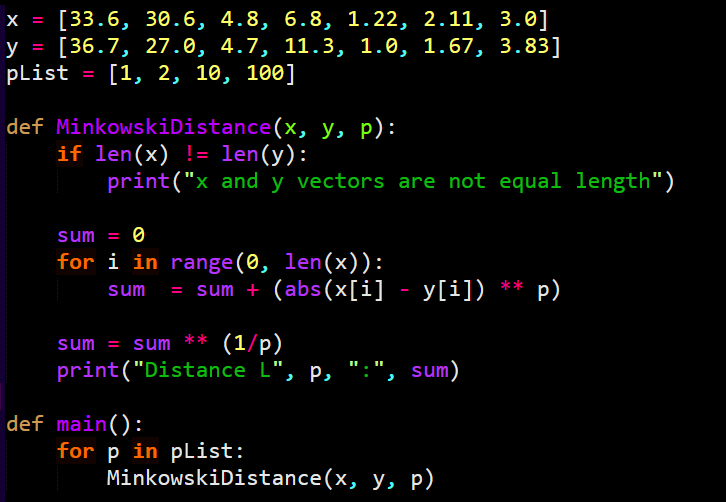
\includegraphics[scale=0.4]{codeSnippet.png}
\end{figure} \\
\textbf{a. } $L1$ distance $=12.79$ \\
\textbf{b. } $L2$ distance $=6.615$ \\
\textbf{c. } $L10$ distance $=4.556$ \\
\textbf{d. } $L100$ distance $=4.5$ \\\\
\textbf{e. } after adding the constant vector the new vectors were\\
$x1 = [38.6, 35.6, 6.8, 8.8, 1.72, 2.21, 4.0]$ \\
$x2 = [41.7, 32.0, 6.7, 13.3, 1.5, 1.77, 4.83]$ \\\\
the distance values remained the same with \\
$L1$ distance $=12.79$ \\
$L2$ distance $=6.615$ \\
$L_{10}$ distance $=4.556$ \\
$L_{100}$ distance $=4.5$ \\
\newpage
When using the constant $k=2$ the new vectors will be\\
$x1 = [67.2, 61.2, 9.6, 13.6, 2.44, 4.22, 6.0]$ \\
$x2 = [73.4, 54.0, 9.4, 22.6, 2.0, 3.34, 7.66]$ \\
All the distances end up changing \\
$L1$ distance $=25.58$ \\
$L2$ distance $=13.23$ \\
$L_{10}$ distance $=9.1126$ \\
$L_{100}$ distance $=9.0$ \\ \\

\subsection*{Problem 4}
\textbf{a. } P(\textit{grade}|\textit{class, effort}) \\
\textbf{Class}: 165B \textbf{Effort}: small \\
A = 0, B = $\frac{1}{6}$, C = $\frac{1}{6}$, D = $\frac{1}{3}$, F = $\frac{1}{3}$ \\
\textbf{Class}: 165B \textbf{Effort}: medium \\
A = $\frac{5}{29}$, B = $\frac{10}{29}$, C = $\frac{10}{29}$, D = $\frac{4}{29}$, F = 0 \\
\textbf{Class}: 165B \textbf{Effort}: large \\
A = $\frac{20}{41}$, B = $\frac{15}{41}$, C = $\frac{5}{41}$, D = $\frac{1}{41}$, F = 0 \\\\
\textbf{Class}: Basketweaving \textbf{Effort}: small \\
A = $\frac{1}{3}$, B = $\frac{1}{3}$, C = $\frac{1}{3}$, D = 0, F = 0 \\
\textbf{Class}: Basketweaving \textbf{Effort}: medium \\
A = $\frac{4}{7}$, B = $\frac{2}{7}$, C = $\frac{1}{7}$, D = 0, F = 0 \\
\textbf{Class}: Basketweaving \textbf{Effort}: large \\
A = $\frac{6}{7}$, B = $\frac{1}{7}$, C = 0, D = 0, F = 0 \\
\newpage
\textbf{b. } \\
\begin{table}[!h]
\begin{tabular}{|l|l|l|l|}
\hline
  & Small & Medium & Large \\ \hline
A & 50    & 125    & 250   \\ \hline
B & 75    & 100    & 100   \\ \hline
C & 75    & 75     & 25    \\ \hline
D & 50    & 20     & 5     \\ \hline
F & 50    & 0      & 0     \\ \hline
\end{tabular}
\end{table} \\
\textbf{Effort: } Small \\
A = $\frac{10}{200}$, B = $\frac{15}{200}$, C = $\frac{15}{200}$, D = $\frac{10}{200}$, F = $\frac{10}{200}$ \\
\textbf{Effort: } Medium \\
A = $\frac{25}{200}$, B = $\frac{20}{200}$, C = $\frac{15}{200}$, D = $\frac{4}{200}$, F = 0 \\
\textbf{Effort: } Large \\
A = $\frac{50}{200}$, B = $\frac{20}{200}$, C = $\frac{5}{200}$, D = $\frac{1}{200}$, F = 0 \\\\
\textbf{c. }\\
Using the table from part \textbf{b.}, sum the 3 different efforts and divide them by the total\\
Small = $\frac{300}{1000} \rightarrow 0.3$, Medium = $\frac{320}{1000} \rightarrow 0.32$, Large = $\frac{380}{1000} \rightarrow 0.38 $ \\\\
\textbf{d. } \\
P(A|165B) = P(A and 165B)/P(165B) = $\frac{1}{4}$ \\
P(A|bascketweaving) = P(A and bascketweaving)/P(bascketweaving) = $\frac{3}{5}$ \\

\subsection*{Problem 5}
\textbf{a. } \\
\begin{table}[h!]
\begin{tabular}{|l|l|l|}
\hline
                     & Labeled Spam & Labeled Non-spam \\ \hline
Detected as Spam     & 1750(TP)     & 250(FN)          \\ \hline
Detected as Non-spam & 250(FP)      & 7750(TN)         \\ \hline
\end{tabular}\\
\end{table}\\
\textbf{b. } false positive rate = $\frac{FP}{N} = \frac{250}{8000} = \frac{1}{32}$\\
\textbf{c. } false negative rate = $\frac{FN}{P} = \frac{250}{2000} = \frac{1}{8}$\\
\textbf{d. } error rate = $\frac{FP + FN}{P + N} = \frac{250 + 250}{2000 + 8000} = \frac{500}{10000} = \frac{1}{20}$\\
\textbf{e. } precision = $\frac{TP}{TP+FP} = \frac{1750}{1750 + 250} = \frac{1750}{2000} = \frac{7}{8}$\\
\textbf{f. } accuracy = 1 - precision = $1 - \frac{1}{20} = \frac{19}{20}$\\
\newpage

\subsection*{Problem 6}
\textbf{a. } 9 ranking errors \\
\textbf{b. } ranking error = $\frac{9}{12 \cdot 13} = 0.058$ \\
\textbf{c. } ranking accuracy = 1 - ranking error = $1 - 0.058 = 0.942$ 

\subsection*{Problem 7}
\subsection*{a. }
\begin{figure}[h!]
	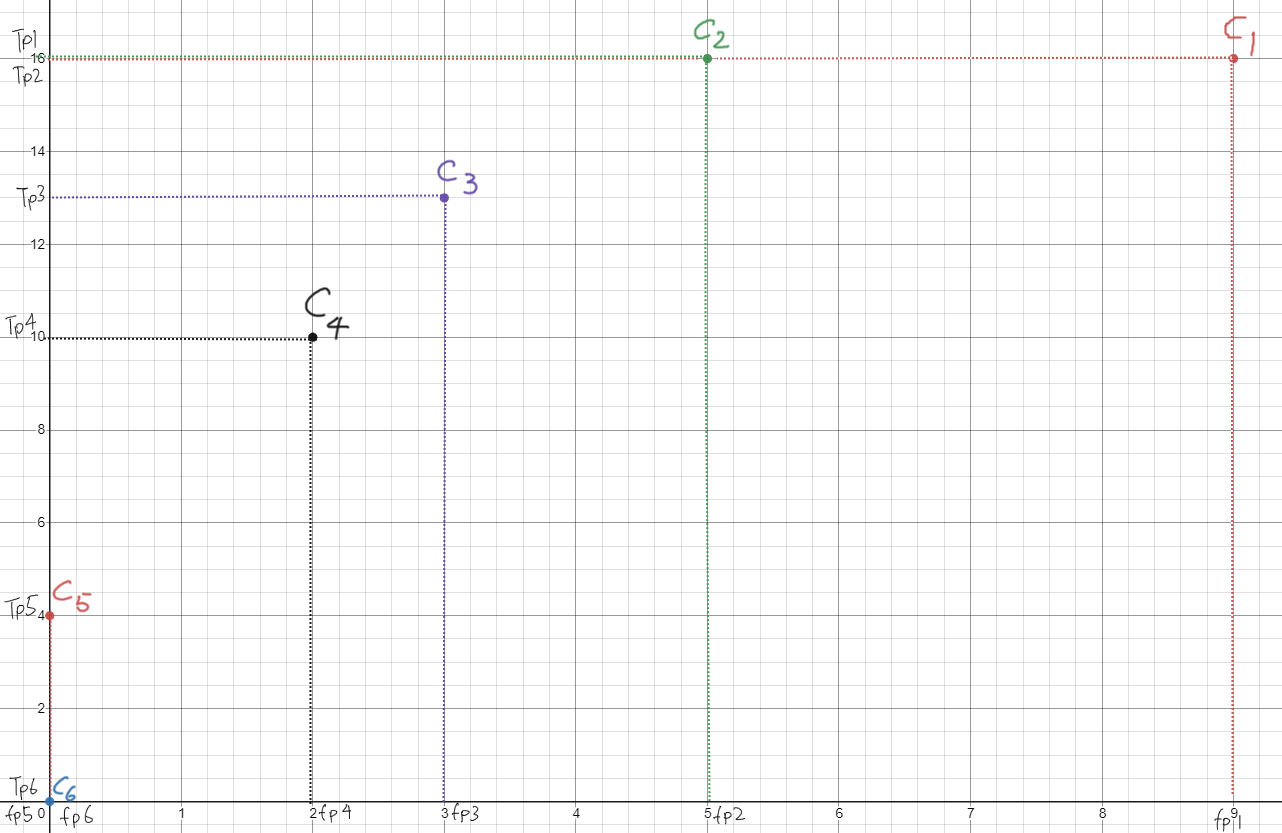
\includegraphics[scale=0.4]{coveragePlot.png}
\end{figure} 
\newpage
\subsection*{b. }
\begin{figure}[h!]
	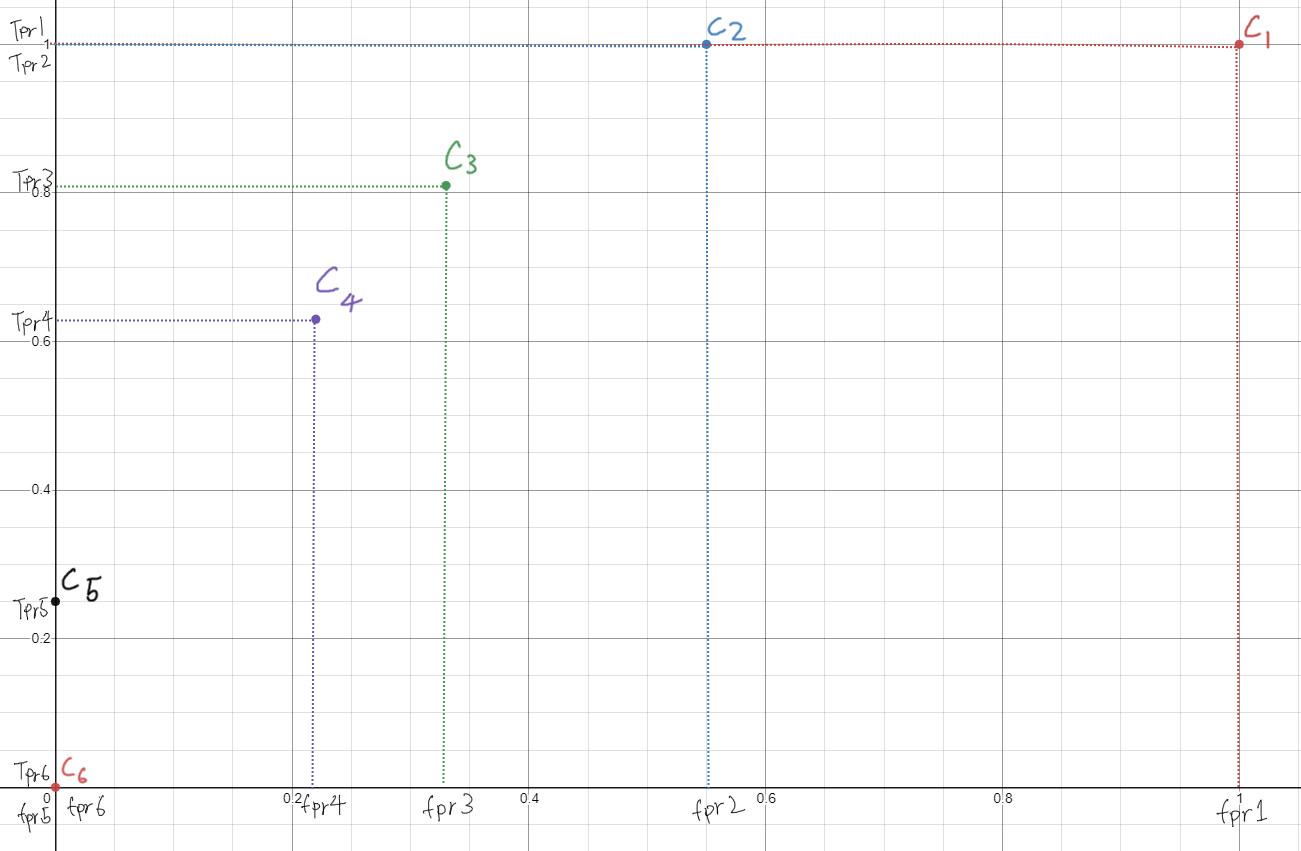
\includegraphics[scale=0.4]{ROCplot.png}
\end{figure} 

\subsection*{c. } 
\textbf{Highest:} C2 = $\frac{20}{25}$ \textbf{Lowest:} C6 = $\frac{9}{25}$ 
\subsection*{d. } 
\textbf{Highest:} C5 = 1 \textbf{Lowest:} C6 = 0 
\subsection*{e. } 
\textbf{Highest:} C1 and C2 \textbf{Lowest:} C6 = 0 
\subsection*{f. } 
C1 and C2
\subsection*{g. } 
C5 and C6
\end{document}









